% Created by tikzDevice version 0.12.3.1 on 2021-07-11 22:19:22
% !TEX encoding = UTF-8 Unicode
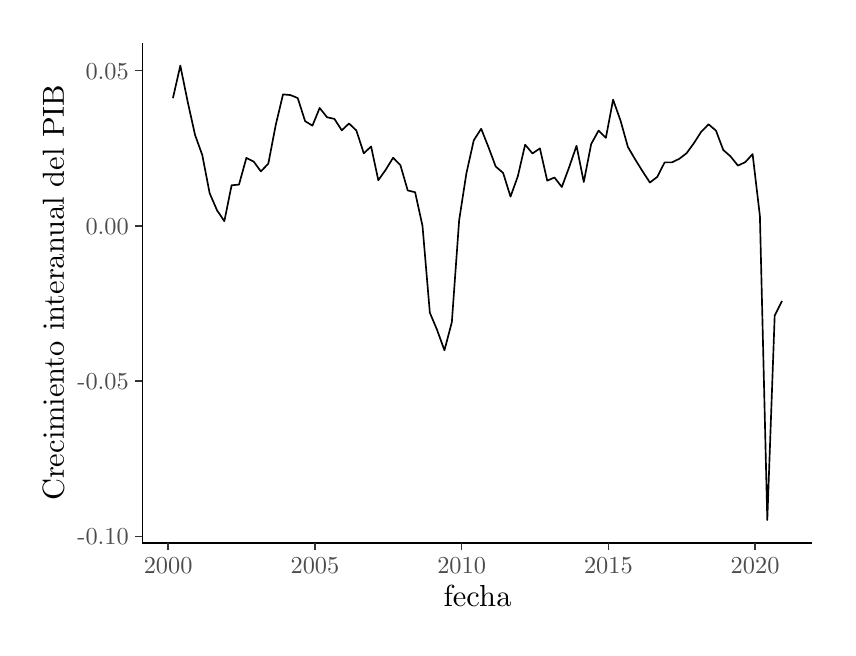
\begin{tikzpicture}[x=1pt,y=1pt]
\definecolor{fillColor}{RGB}{255,255,255}
\path[use as bounding box,fill=fillColor,fill opacity=0.00] (0,0) rectangle (289.08,216.81);
\begin{scope}
\path[clip] (  0.00,  0.00) rectangle (289.08,216.81);
\definecolor{drawColor}{RGB}{255,255,255}
\definecolor{fillColor}{RGB}{255,255,255}

\path[draw=drawColor,line width= 0.6pt,line join=round,line cap=round,fill=fillColor] (  0.00,  0.00) rectangle (289.08,216.81);
\end{scope}
\begin{scope}
\path[clip] ( 41.49, 30.69) rectangle (283.58,211.31);
\definecolor{fillColor}{RGB}{255,255,255}

\path[fill=fillColor] ( 41.49, 30.69) rectangle (283.58,211.31);
\definecolor{drawColor}{RGB}{0,0,0}

\path[draw=drawColor,line width= 0.6pt,line join=round] ( 52.49,191.34) --
	( 55.16,203.10) --
	( 57.83,189.99) --
	( 60.48,178.05) --
	( 63.09,170.79) --
	( 65.76,156.97) --
	( 68.43,150.80) --
	( 71.07,146.89) --
	( 73.69,159.86) --
	( 76.36,160.10) --
	( 79.03,169.75) --
	( 81.67,168.42) --
	( 84.28,164.87) --
	( 86.96,167.69) --
	( 89.63,181.62) --
	( 92.27,192.70) --
	( 94.91,192.46) --
	( 97.58,191.38) --
	(100.25,183.03) --
	(102.90,181.41) --
	(105.51,187.79) --
	(108.18,184.44) --
	(110.85,183.84) --
	(113.49,179.71) --
	(116.11,182.19) --
	(118.78,179.64) --
	(121.45,171.41) --
	(124.09,173.87) --
	(126.70,161.68) --
	(129.38,165.47) --
	(132.05,169.81) --
	(134.69,167.10) --
	(137.33,157.99) --
	(140.00,157.35) --
	(142.67,145.18) --
	(145.32,113.82) --
	(147.93,107.62) --
	(150.60,100.22) --
	(153.27,110.40) --
	(155.91,147.22) --
	(158.53,164.19) --
	(161.20,176.12) --
	(163.87,180.28) --
	(166.51,173.63) --
	(169.12,166.63) --
	(171.80,164.32) --
	(174.47,155.76) --
	(177.11,163.08) --
	(179.75,174.53) --
	(182.42,171.36) --
	(185.09,173.19) --
	(187.74,161.52) --
	(190.35,162.67) --
	(193.02,159.24) --
	(195.69,166.48) --
	(198.33,174.13) --
	(200.95,161.05) --
	(203.62,174.76) --
	(206.29,179.62) --
	(208.93,177.00) --
	(211.54,190.78) --
	(214.22,183.25) --
	(216.89,173.69) --
	(219.53,169.20) --
	(222.17,164.93) --
	(224.84,160.86) --
	(227.51,162.89) --
	(230.16,168.13) --
	(232.77,168.12) --
	(235.44,169.41) --
	(238.11,171.46) --
	(240.75,175.10) --
	(243.37,179.18) --
	(246.04,181.88) --
	(248.71,179.61) --
	(251.35,172.61) --
	(253.96,170.31) --
	(256.64,166.98) --
	(259.31,168.22) --
	(261.95,171.12) --
	(264.59,148.74) --
	(267.26, 38.90) --
	(269.93,112.73) --
	(272.58,118.04);
\end{scope}
\begin{scope}
\path[clip] (  0.00,  0.00) rectangle (289.08,216.81);
\definecolor{drawColor}{RGB}{0,0,0}

\path[draw=drawColor,line width= 0.6pt,line join=round] ( 41.49, 30.69) --
	( 41.49,211.31);
\end{scope}
\begin{scope}
\path[clip] (  0.00,  0.00) rectangle (289.08,216.81);
\definecolor{drawColor}{gray}{0.30}

\node[text=drawColor,anchor=base east,inner sep=0pt, outer sep=0pt, scale=  0.88] at ( 36.54, 29.88) {-0.10};

\node[text=drawColor,anchor=base east,inner sep=0pt, outer sep=0pt, scale=  0.88] at ( 36.54, 86.01) {-0.05};

\node[text=drawColor,anchor=base east,inner sep=0pt, outer sep=0pt, scale=  0.88] at ( 36.54,142.13) {0.00};

\node[text=drawColor,anchor=base east,inner sep=0pt, outer sep=0pt, scale=  0.88] at ( 36.54,198.25) {0.05};
\end{scope}
\begin{scope}
\path[clip] (  0.00,  0.00) rectangle (289.08,216.81);
\definecolor{drawColor}{gray}{0.20}

\path[draw=drawColor,line width= 0.6pt,line join=round] ( 38.74, 32.92) --
	( 41.49, 32.92);

\path[draw=drawColor,line width= 0.6pt,line join=round] ( 38.74, 89.04) --
	( 41.49, 89.04);

\path[draw=drawColor,line width= 0.6pt,line join=round] ( 38.74,145.16) --
	( 41.49,145.16);

\path[draw=drawColor,line width= 0.6pt,line join=round] ( 38.74,201.28) --
	( 41.49,201.28);
\end{scope}
\begin{scope}
\path[clip] (  0.00,  0.00) rectangle (289.08,216.81);
\definecolor{drawColor}{RGB}{0,0,0}

\path[draw=drawColor,line width= 0.6pt,line join=round] ( 41.49, 30.69) --
	(283.58, 30.69);
\end{scope}
\begin{scope}
\path[clip] (  0.00,  0.00) rectangle (289.08,216.81);
\definecolor{drawColor}{gray}{0.20}

\path[draw=drawColor,line width= 0.6pt,line join=round] ( 50.75, 27.94) --
	( 50.75, 30.69);

\path[draw=drawColor,line width= 0.6pt,line join=round] (103.80, 27.94) --
	(103.80, 30.69);

\path[draw=drawColor,line width= 0.6pt,line join=round] (156.81, 27.94) --
	(156.81, 30.69);

\path[draw=drawColor,line width= 0.6pt,line join=round] (209.83, 27.94) --
	(209.83, 30.69);

\path[draw=drawColor,line width= 0.6pt,line join=round] (262.85, 27.94) --
	(262.85, 30.69);
\end{scope}
\begin{scope}
\path[clip] (  0.00,  0.00) rectangle (289.08,216.81);
\definecolor{drawColor}{gray}{0.30}

\node[text=drawColor,anchor=base,inner sep=0pt, outer sep=0pt, scale=  0.88] at ( 50.75, 19.68) {2000};

\node[text=drawColor,anchor=base,inner sep=0pt, outer sep=0pt, scale=  0.88] at (103.80, 19.68) {2005};

\node[text=drawColor,anchor=base,inner sep=0pt, outer sep=0pt, scale=  0.88] at (156.81, 19.68) {2010};

\node[text=drawColor,anchor=base,inner sep=0pt, outer sep=0pt, scale=  0.88] at (209.83, 19.68) {2015};

\node[text=drawColor,anchor=base,inner sep=0pt, outer sep=0pt, scale=  0.88] at (262.85, 19.68) {2020};
\end{scope}
\begin{scope}
\path[clip] (  0.00,  0.00) rectangle (289.08,216.81);
\definecolor{drawColor}{RGB}{0,0,0}

\node[text=drawColor,anchor=base,inner sep=0pt, outer sep=0pt, scale=  1.10] at (162.53,  7.64) {fecha};
\end{scope}
\begin{scope}
\path[clip] (  0.00,  0.00) rectangle (289.08,216.81);
\definecolor{drawColor}{RGB}{0,0,0}

\node[text=drawColor,rotate= 90.00,anchor=base,inner sep=0pt, outer sep=0pt, scale=  1.10] at ( 13.08,121.00) {Crecimiento interanual del PIB};
\end{scope}
\end{tikzpicture}
